\documentclass[12pt]{article}

%%    LES PACKAGES
\usepackage{import}
\usepackage{enumitem}%Pour faire des listes à puces stylés.
\usepackage{pifont} %Pour changer les symboles dans les listes à puces.
\usepackage{stmaryrd}%Pour les intervalles discrets.
\usepackage{amsmath}
\usepackage{amsfonts}
\usepackage{amssymb}
\usepackage{amsthm}
\usepackage{esint}
\usepackage[most,many,breakable]{tcolorbox}
\usepackage{graphicx}
\usepackage{color}
\usepackage{nicefrac}
\usepackage{mathtools}
\usepackage{xcolor}
\usepackage{awesomebox}
\usepackage{cancel}
\usepackage{setspace}
\usepackage{varwidth}
\usepackage{mathrsfs}
\usepackage{listings}
\usepackage{float}
\usepackage{wrapfig}
\usepackage[frenchb]{babel}
\usepackage[left=1cm, right=1cm, top=1cm, bottom=1.5cm]{geometry}



%%    MISE EN PAGE
%\pagecolor{black}
%\color{white}

% Pour Code 
\lstset{
	language=Python,                % Langage du code
	basicstyle=\ttfamily\small,     % Style de base
	keywordstyle=\color{blue},      % Mots-clés
	stringstyle=\color{orange},     % Chaînes de caractères
	commentstyle=\color{gray},      % Commentaires
	numbers=left,                   % Numéros de ligne
	numberstyle=\tiny\color{gray}, % Style des numéros de ligne
}

\definecolor{Aquamarine}{HTML}{00B5BE}
\normalfont
\DeclareMathSizes{10}{9}{7}{5}
\baselineskip=12pt


%%%%%%%%%%%%%%%%%%%%%%%%%%%%%%
%%    LES ENVIRONNEMENTS
%%%%%%%%%%%%%%%%%%%%%%%%%%%%%%
\newtheoremstyle{saav}
{ }
{ }
{\normalfont}
{}
{\bfseries\large}
{:}
{\newline}
{ }
\theoremstyle{saav}

\newtheorem{definition}{Définition}[section]
\newtheorem{propriete}{Propriétés}
\newtheorem{theoreme}{Théorème}
\newtheorem*{proposition}{Proposition}
\newtheorem*{preuve}{Preuve}
\newtheorem*{remark}{Remarque}
\newtheorem{exercice}{Exercice}
\newcommand{\defi}{\begin{tcolorbox}[title=Définition, colframe=red!75!black, colback=red!10!white]}
\newcommand{\prop}{\begin{tcolorbox}[title=Propriété, colframe=blue!85!black, colback=blue!10!white]}
\newcommand{\impo}{\begin{tcolorbox}[title=Points importants, colframe=black!0!black, colback=black!0!white]}
\newcommand{\close}{\end{tcolorbox}}
\newtcolorbox{mybox}{colback=black!5!white,colframe=black!75!black}


%% LES MACROS
\newcommand{\summ}[2]{\sum_{#1}^{#2}}
\newcommand{\dps}{\displaystyle}
\newcommand{\sk}{\smallskip}
\newcommand{\bk}{\bigskip}
\newcommand{\jump}{~~}
\newcommand{\acc}[1]{\hspace{-0.05cm}\left\{#1 \right\}}
\newcommand{\parr}[1]{\hspace{-0.05cm}\left(#1 \right)}
\newcommand{\rect}[1]{\left[ #1 \right]}
\newcommand{\braks}[1]{\hspace{-0.05cm}\llbracket#1 \rrbracket}
\newcommand{\abs}[1]{\hspace{-0.05cm}\left\lvert#1 \right\rvert}
\newcommand{\eq}{\Leftrightarrow}
\newcommand{\mc}[1]{\mathcal{#1}}
\newcommand{\mb}[1]{\mathbb{#1}}
\newcommand{\mr}[1]{\mathscr{#1}}
\newcommand{\Ra}{\Rightarrow}
\newcommand{\projet}[3]{p_{#1\Vert #2}(#3)}
\newcommand{\projeet}[2]{p_{#1\Vert #2}}
\newcommand{\ra}{\rightarrow}
\newcommand{\lra}{\longrightarrow}
\newcommand{\la}{\leftarrow}
\newcommand{\exs}{\exists}
\newcommand{\fonction}[3]{#1:#2\longrightarrow#3}
\newcommand{\famille}[3]{#1_#2,\dots,#1_#3}
\newcommand{\transpose}[1]{{}^{t\!}#1}
\newcommand{\longvec}[1]{\overrightarrow{#1}}

%% MACRO POUR LES MBOX
\newcommand{\tw}{\textwidth}
\newcommand{\blue}{\color{blue}}
\newcommand{\red}{\color{red}}
\newcommand{\green}{\color{green}}
\newcommand{\blackt}{\color{black}}


\title{Modélisation du Stockage du Dioxyde de Carbone dans les Forêts}
\author{Ben Khalifa Emna, Giovanni Honakoko, Ziad Zineb }
\date{Projet MAM3 Analyse Numérique 2 \\ 2024-2025}
	

%NOM BIBLIOGRAPHIE
%	ARTICLE 1 : friedlingstein2006climate
%	ARTICLE 2 : jenkinson1977turnover
%	ARTICLE 3 : manzoni2009soil
%	ARTICLE 4 : into1988division
%	ARTICLE 5 : sitch2003evaluation
	
\begin{document}
		\maketitle
		\begin{figure}[h]
			\centering
			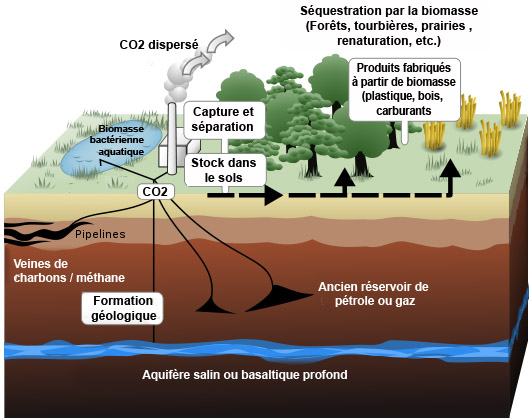
\includegraphics[width=0.6\linewidth]{images/schema_puit_de_carbone.jpg}
		\end{figure}
			\begin{abstract}
			\noindent
			Ce projet s'intéresse à la modélisation mathématiques des échanges de carbone entre l'atmosphère, les arbres et les sols forestiers. Dans un contexte de changement climatique où la séquestration naturelle du CO\textsubscript{2} devient un enjeu majeur, nous développons un modèle dynamique basé sur des \textbf{EDO} (Équations Différentielles Ordinaires). L'objectif est d'analyser l'impact des différents paramètres écologiques sur les flux de carbone et d'évaluer numériquement les équilibres du système à l'aide de méthodes numériques avancées vu en cours.
		\end{abstract}
		\begin{figure}[b]
			\raggedleft
			
\includegraphics[width=0.5\linewidth]{images/logo_pns.png}
		\end{figure}
		\newpage
		\tableofcontents
	
		\rule{\linewidth}{0.4pt}
		
	\setlength{\intextsep}{12pt plus 2pt minus 2pt} % Espace autour des figures
	\setlength{\textfloatsep}{12pt plus 2pt minus 2pt} % Espace entre figures
	\setlength{\parindent}{0pt} % Supprime l'indentation de tous les paragraphes
	\section{Introduction}
	\subsection{Contexte et enjeux actuels}
	Le réchauffement climatique, principalement dû à l'augmentation des concentrations atmosphériques de CO\textsubscript{2}, représente l'un des défis majeurs du XXI\textsuperscript{e} siècle. Selon le GIEC, les écosystèmes terrestres, et particulièrement les forêts, séquestrent environ 30\% des émissions anthropiques annuelles de CO2 \cite{friedlingstein2006climate}. 
	Cette capacité naturelle de stockage fait des forêts un élément clé dans les stratégies d'atténuation du changement climatique.
	
	Cependant, cette fonction de \og \emph{puits de carbone} \fg \hspace{1mm} qui capte naturellement le CO\textsubscript{2} par photosynthèse et le stocke dans le bois, les sols, les sédiments est influencée par de nombreux facteurs :
	\begin{itemize}[label*=\textbullet]
		\item Les paramètres physiologiques des arbres (taux de croissance, respiration)
		\item Les processus de décomposition dans les sols
		\item Les perturbations naturelles (incendies, sécheresses)
		\item Les activités humaines (déforestation, gestion forestière)
	\end{itemize}
	
	\textit{,voir} \cite{jenkinson1977turnover}, \cite{manzoni2009soil}, \cite{into1988division}, \cite{sitch2003evaluation}
	
	\subsection{Objectifs du projet}
	Dans ce contexte, notre projet vise à :
	\begin{itemize}[label*=\textbullet]
		\item Développer un modèle mathématiques simplifié des flux de carbone forestier
		\item Implémenter des méthodes numériques pour résoudre le système d'équations
		\item Analyser la sensibilité du système aux différents paramètres écologiques
		\item Proposer des améliorations pour un modèle plus réaliste
	\end{itemize}
	
	\section{Théorie}
	\subsection{Description du modèle}
	Nous considérons trois compartiments principaux :
	\begin{itemize}
		\item $C_A(t)$ : Carbone atmosphérique (CO\textsubscript{2})
		\item $C_T(t)$ : Carbone stocké dans la biomasse arborée
		\item $C_S(t)$ : Carbone stocké dans les sols
	\end{itemize}
	
	Les échanges entre ces compartiments sont régis par le système d'équations différentielles suivant :
	
	\begin{align}
		\frac{dC_A}{dt} &= -S(C_T) + \beta C_T + \delta C_S \label{eq:ca} \\
		\frac{dC_T}{dt} &= S(C_T) - \beta C_T - \delta C_T - \gamma C_T \label{eq:ct} \\
		\frac{dC_S}{dt} &= \gamma C_T - \delta C_S + \delta C_T \label{eq:cs}
	\end{align}
	
	où :
	\begin{itemize}
		\item $S(C_T) = \alpha C_T (1 - \frac{C_T}{K})$ : Séquestration photosynthétique (modèle logistique)
		\item $\beta$ : Taux de respiration des arbres vers l'atmosphère
		\item $\delta$ : Taux d'échange arbres-sols et sols-atmosphère
		\item $\gamma$ : Taux de production de litière
		\item $K$ : Capacité maximale de stockage arboré
	\end{itemize}
	
	\section{Méthodes Numériques}
	Nous avons considéré comme conditions initiales :

	\bk
	
	
	\noindent
	\begin{minipage}[t]{0.3\textwidth}
	\begin{itemize}
		\item $\beta = 0.1$
		\item $\delta = 0.01$
		\item $\gamma = 0.03$
		\item $\alpha = 0.04$
		\item $K = 500.0$
	\end{itemize}
	\end{minipage}
	\hspace{0.01\textwidth}% espace horizontal entre les colonnes
	\begin{minipage}[t]{0.3\textwidth}
		\begin{itemize}
			\item \texttt{x0}$= \begin{bmatrix}
				3250\\
				500\\
				5500
			\end{bmatrix}$
			\item \texttt{t0} $= 0$
			\item \texttt{tf}$=600$
			\item  \texttt{N}$=6000$
		\end{itemize}
	\end{minipage}
	\bk
	
	Pour résoudre ce système, nous avons tenté d'implémenter les méthodes suivantes:
	\begin{itemize}[label*=\textbullet]
		\item \textbf{Dichotomie}
%		, pour f(x)=0
%		\begin{itemize}
%			\item L'équation (2) devient : $f(C_T)=0$
%			\item L'équation (3) devient : $f(C_S)=0$
%			\item $C_A$ est obtenue à l'aide des résultats des deux autres équations
%		\end{itemize}
%		Résultats obtenus :
%		\begin{itemize}
%			\item CT = 25.00000248551369
%			\item CS = 58.33336782455443
%			\item CA = 1.4821291580702223e-06
%		\end{itemize}
		
		\item \textbf{Newton implicite}
		
		\item \textbf{Newton explicite}
		
		\item \textbf{Euler explicite} 
		
		\item \textbf{Euler implicite}
		
		\item \textbf{Jacobi}
		\item \textbf{Gauss Seidel}
		\item \textbf{SOR}
		
	\end{itemize}
	Au départ, nous avons eu du mal à se positionner par rapport au problème et dans sa formalisation avant de proposer des pistes de résolution.
	
	
	Nous nous sommes rendu compte assez vite que les méthodes de résolution de systèmes linéaires ne s'appliquaient pas. Puisque notre système est de la forme : \begin{equation*}
		A(t)x = b
	\end{equation*}
	Donc c'est un système non linéaire. Ainsi les méthodes de Jacobi, Gauss-Seidel et SOR ne sont pas adéquates.
	\sk 
	
	
	Parmi les méthodes de résolution d'équations non linéaires, nous avons conservé uniquement la méthode de Newton explicite, car c'était la plus optimale en pratique. On expliquera plus tard l'utilité d'une telle méthode.
	\bk 
	
	
	
	Par la suite nous avons chercher à résoudre vectoriellement notre système par des méthodes de résolution numérique d'EDO comme Adam-Bashforth, Runge-Kutta et Euler (explicite et implicite).
	
	Pour cela nous avons créé une fonction \texttt{systeme} qui renvoie un tableau avec les valeurs de $\frac{\mathrm{d}C_{A}}{d\mathrm{t}}, \frac{\mathrm{d}C_{T}}{\mathrm{t}},\frac{\mathrm{d}C_{S}}{d\mathrm{t}}$, où : 
	\begin{equation*}
		x = \begin{bmatrix}
			C_{A}\\
			C_{T}\\
			C_{S}
		\end{bmatrix} , 
		\quad
		 f(t,x) = \begin{bmatrix}
		\nicefrac{\mathrm{d}C_{A}}{d\mathrm{t}}\\
		\nicefrac{\mathrm{d}C_{T}}{d\mathrm{t}}\\
		\nicefrac{\mathrm{d}C_{S}}{d\mathrm{t}}
		\end{bmatrix}
	\end{equation*}
	
	\section{Méthode Explicite}
		\subsection{Euler Explicite}
		Sur un intervalle discrétiser, on construit à chaque pas de temps la suite $(y_{n})_{n \in \mb{N}}$ via la formule d'itérative :
		\begin{equation}
			y_{n+1}=y_n+hf(t_n,y_n)
			\label{eq:euler_exp}
		\end{equation} 
		On a uniquement besoin d'une boucle \texttt{for} afin de calculer les itérés de la suite et ce, pour chacune des EDO dans notre système.
		
		
	

		\subsection{Adams-Bashforth (Ordre 2)}
			De façon analogue à Euler explicite, la méthode d'Adams-Bashforth permet de construire la suite $(y_{n})_{n \in \mb{N}}$ convergeant vers la solution de l'EDO. C'est une méthode dite de \textbf{multistep} car elle utilise l'expression des termes précédents pour le calcul du prochain terme, on le remarque par l'expression des termes de la suite : 
			\begin{equation}
				y_{n+1} = y_{n} + \frac{h}{2}\rect{3 f(t_{n},y_{n}) - f(t_{n-1}, y_{n-1})}\label{eq:AB}
			\end{equation}
			Pour initialiser cette méthode on utilise la méthode d'Euler explicite, puis on peut calculer le reste des itérés via une boucle \texttt{for} via la formule itérative [\ref{eq:AB}].
		\subsection{Runge-Kutta (Ordre 2)}
			La méthode de Runge-Kutta d'ordre 2 (méthode de Heun) permet de résoudre des EDO classiques, c'est une méthode par paliers tout comme les méthodes précédentes, donc qui fonctionne par pas de temps régulier.  
			Cette méthode se définie par : 
			\begin{align*}
				k_{1}&= f(t_{n},y_{n})
				\\
				k_{2}&= f(t_{n} + h, y_{n} + hk_{1})
				\\
				y_{n+1} &= y_{n} + \frac{h}{2}(k_{1} + k_{2})
			\end{align*}
			
			où $k_{1}$ est la pente initiale, et $y_{n} + hk_{1}$ est une estimation grossière de la valeur future de la solution. Par la suite $k_{2}$ est l'estimation de la pente en ce nouveau point et l'itéré suivant de la suite $(y_{n})_{n \in \mb{N}}$ est la combinaison de ces deux pentes.
			
			Le tableau de Butcher correspondant est : 
			 \[
			 \begin{array}{c|cc}
			 	0 & 0 & 0 \\
			 	1 & 1 & 0 \\
			 	\hline
			 	& \nicefrac{1}{2} & \nicefrac{1}{2}
			 \end{array}
			 \]
			 	 
		
		\subsection{Newton explicite}
		La méthode de Newton permet de résoudre des équations non linéaires, du type $f(x^*)=0$ pour un $x^*$ : la solution recherchée. On construit une suite $(x_{n})_{n \in \mb{N}}$ de façon à approcher la solution par une succession de construction de tangente. 
		
		
			\textbf{Formule en dimension 1 }: 
			\begin{equation}
				x_{n+1} = x_{n} - 	\dfrac{f(x_{n})}{f'(x_{n})}
			\end{equation}
			\textbf{Formule en dimension $n$ }: 
			\begin{equation*}
				X^{(n+1)} = X^{(n)} - 	\rect{J_{f}\parr{X^{(n)}}}^{-1}\cdot f(X^{(n)})
			\end{equation*}
			Au départ nous avions imaginé notre système d'équation comme : 
			\begin{equation*}
				f(x) = 0_{E} \iff \begin{cases}
					f_{1}(x)=0\\
					f_{2}(x)=0\\
					f_{3}(x)=0
				\end{cases} \text{, où $x = (C_{A},C_{T},C_{S})^{T}$ }
			\end{equation*}
			
			
			Nous avons essayé de résoudre le système avec la méthode de Newton en $n$ dimension, or la matrice jacobienne :
			\begin{equation*}
				J_{f}(X^{(n)}) = \begin{bmatrix}
					0 & - \alpha\rect{\parr{1 - \frac{C_{T}}{K}} + C_{T} \parr{1 - \frac{1}{K}}} + \beta& \delta \\
					0& \alpha\rect{\parr{1 - \frac{C_{T}}{K}} + C_{T}\parr{1 - \frac{1}{K}}} - \parr{\beta + \delta+\gamma}&0 \\
					0&\gamma + \delta  & - \delta 
				\end{bmatrix}
			\end{equation*}
			étant singulière, il était impossible de continuer avec un tel procédé.
			
	
	
	
	
	\section{Méthode Implicite}
		\subsection{Euler Implicite}
		Cette méthode repose presque sur le même principe que sa version explicite, l'expression de $(y_{n})_{n\in \mb{N}}$ étant donné par :
			\begin{equation}
				y_{n+1}=y_n+hf(t_{n+1},y_{n+1})
				\label{eq:euler_imp}
			\end{equation}
		Par une telle méthode notre système devient : 
		\begin{equation*}
			\begin{cases}
				C_{A}^{(n+1)} &= C_{A}^{(n)} + \Delta t \rect{- S \parr{C_{T}^{(n+1)}} + \beta C_{T}^{(n+1)} + \delta C_{S}^{(n+1)} }\\
				
				C_{T}^{(n+1)} &= C_{T}^{(n)} + \Delta t \rect{ S\parr{C_{T}^{(n+1)}} - C_{T}^{(n+1)}(\beta + \gamma + \delta ) }
				\\
				C_{S}^{(n+1)} &= C_{S}^{(n)} + \Delta t  \rect{C_{T}^{(n+1)}(\gamma + \delta) - \delta C_{S}^{(n+1)}}
				
			\end{cases}
		\end{equation*}
		
		Les lignes étant corrélées il faut nécessairement résoudre la ligne $\boldsymbol{2}$ avant de résoudre la $\boldsymbol{3}$, puis la $\boldsymbol{1}$.  Puisque toute les lignes dépendent de $C_{T}^{(n+1)}$.
		D'où :
		\begin{align*}
			C_{T}^{(n+1)} &=  C_{T}^{(n)} + \Delta t \rect{ S\parr{C_{T}^{(n+1)}} - C_{T}^{(n+1)}(\beta + \gamma + \delta ) }
			\\
			&= C_{T}^{(n)} +  \Delta t \rect{ \alpha C_{T}^{(n+1)} \parr{1 - \frac{C_{T}^{(n+1)}}{K}}  - C_{T}^{(n+1)}(\beta + \gamma + \delta ) }
			\\
			C_{T}^{(n+1)}	&= C_{T}^{(n)} + \Delta t \rect{ C_{T}^{(n+1)} (\alpha - (\beta + \gamma + \delta )) - \frac{\alpha}{K}\parr{C_{T}^{(n+1)}}^{2} }
		\end{align*}
		L'équation étant quadratique en $C_{T}^{(n+1)}$, elle est non linéaire on utilisera donc la méthode de Newton (en dimension 1) pour palier à cet effet.
		
		Ainsi on a :
		\begin{equation*}
			F\parr{C_{T}^{(n+1)}} = C_{T}^{(n+1)} + \frac{\alpha}{K}\parr{C_{T}^{(n+1)}}^{2}  - C_{T}^{(n+1)} (\alpha - (\beta + \gamma + \delta )) \Delta t  - C_{T}^{(n)}=0
		\end{equation*}
		en posant $x= C_{T}^{(n+1)}$, il vient que $F(x) = 0$. 
		
		
		D'autre part : 
		\begin{equation*}
			F'(x) = 1 + \frac{2 \alpha \Delta t}{K}x - (\alpha - (\beta+ \gamma + \delta )) \Delta t 
		\end{equation*}
		
		Et on continue à appliquer Newton jusqu'à \texttt{tf} en stockant tous nos résultats dans un vecteurs \texttt{C\_T}. Par la suite on cherche à résoudre la ligne $\boldsymbol{1}$. On a :
		\begin{align*}
			C_{S}^{(n+1)} &= C_{S}^{(n)} + \Delta t \parr{C_{T}^{(n+1)} (\delta + \gamma ) - \delta C_{S}^{(n+1)}}
			\\
			&= C_{S}^{(n)} + x (\delta + \gamma )\Delta t - \delta C_{S}^{(n+1)} \Delta t 
			\\
			C_{S}^{(n+1)} \parr{1 + \delta \Delta t }&= C_{S} + x(\delta + \gamma )\Delta t
			\\
			C_{S}^{(n+1)}&=\frac{C_{S}^{(n)} + x(\delta + \gamma) \Delta t }{1+  \delta \Delta t}
		\end{align*}
		L'équation étant linéaire, nul besoin d'appliquer Newton. On peut calculer directement nos itérés avec une boucle et les stocker dans un vecteur \texttt{C\_S}. 
		
		\bk 
		
		Enfin on peut calculer la valeur de $C_{A}^{(n+1)}$ dans une boucle extérieur à la fonction \texttt{euler\_implicite} grâce à l'expression de $C_{S}^{(n+1)}$ et $x$ que l'on a calculé au préalable. D'où :
		\begin{equation*}
			C_{A}^{(n+1)} = C_{A}^{(n)} - S(x) \Delta t + \delta C_{S}^{(n+1)} \Delta t
		\end{equation*}
		\ding{110}
		
		Une telle résolution nous a mené à traiter le système ligne par ligne là ou pour toute les autres méthodes nous avions pu effectuer le même travail de façon vectoriel et compact au sein d'une même fonction. 
		
	\section{Résultats }
	
	Python possède une fonction \texttt{solve\_ivp} dans la librairie \texttt{scipy.integrate} qui permet de résoudre formellement des EDO, donc on a des solutions très proche des solutions exactes par cet outil. Nous avons donc pris les résultats du code \texttt{solveur.py} comme référence pour nos autres méthodes.
%	\begin{figure}[htpb]
%		\begin{minipage}[t]{0.48\linewidth}
%			\centering 
%			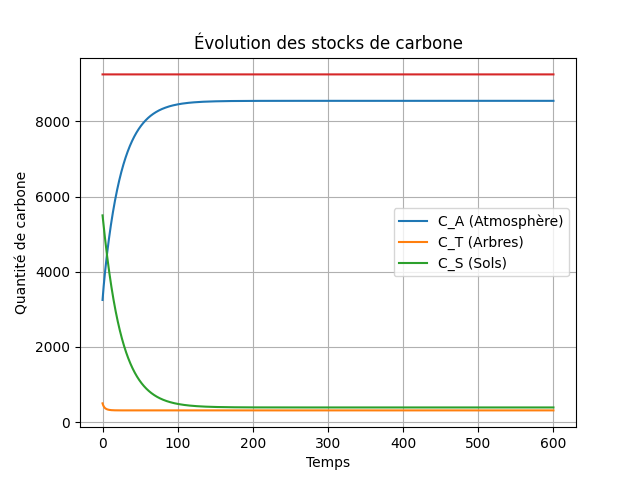
\includegraphics[width=\linewidth]{images/solveur_solutions2.png}
%			\caption{Solutions du solveur}
%		\end{minipage}
%		\hfill 
%		\begin{minipage}[t]{0.48\linewidth}
%			\vspace{0pt}
%			\small 
%			
%			On peut constater qu'au fil du temps les arbres stockeront moins de carbone, les sols également. Il y aura donc plus de carbone dans l'atmosphère en contrepartie. 	
%		\end{minipage}
%		
%	\end{figure}
\begin{figure}[htbp]
	\centering
	\begin{minipage}[t]{0.48\textwidth}
		\vspace{0pt} % Reset crucial
		\centering
		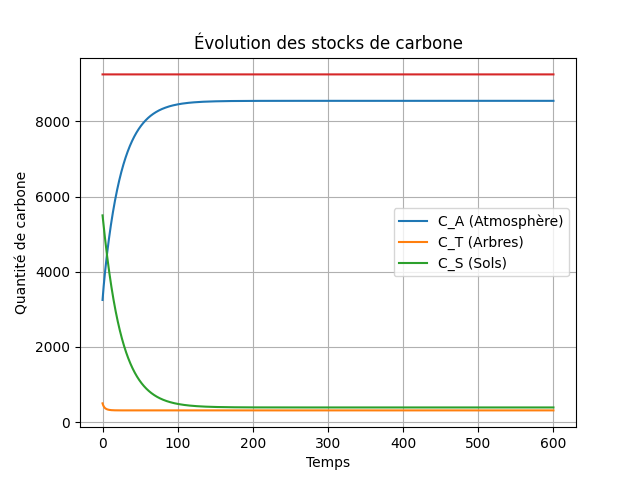
\includegraphics[width=\linewidth]{images/solveur_solutions2.png}
		\caption{Solutions du solveur}
		\label{fig:solveur}
	\end{minipage}% 
	\hfill
	\begin{minipage}[t]{0.48\textwidth}
%		\vspace{0pt}
		\hspace{3mm} 
		\begin{flushleft} 
			\small
			On peut constater qu'au fil du temps les arbres stockeront moins de carbone, les sols également. Il y aura donc plus de carbone dans l'atmosphère en contrepartie.
			
			\textit{ \red La ligne rouge représente la somme des courbes de $C_{A},C_{T}$ et $C_{S}$.}
		\end{flushleft}
	\end{minipage}
\end{figure}

	
	

	\begin{figure}[htbp]
		\centering
		\begin{minipage}{0.48\textwidth}
			\centering
			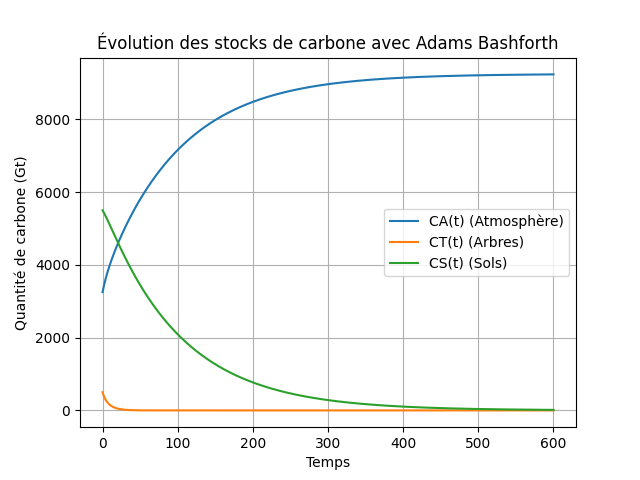
\includegraphics[width=\linewidth]{images/Adams_Bashforth.png}

		\end{minipage}%
		\hfill
		\begin{minipage}{0.48\textwidth}
			\centering
			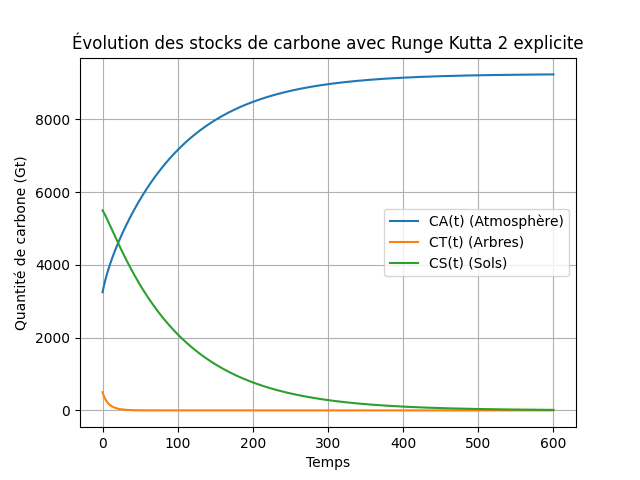
\includegraphics[width=\linewidth]{images/Runge_Kutta_2.png}

		\end{minipage}
		
		\vspace{0.5cm}
		
		\begin{minipage}{0.48\textwidth}
			\centering
			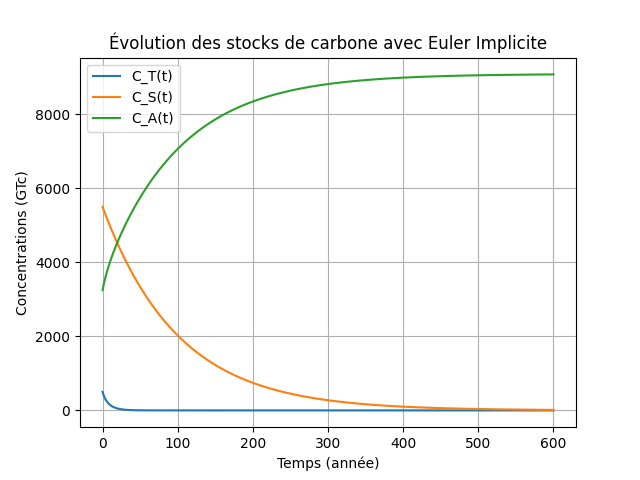
\includegraphics[width=\linewidth]{images/Euler_Implicite.png}

		\end{minipage}
		\begin{minipage}{0.48\textwidth}
			\centering
			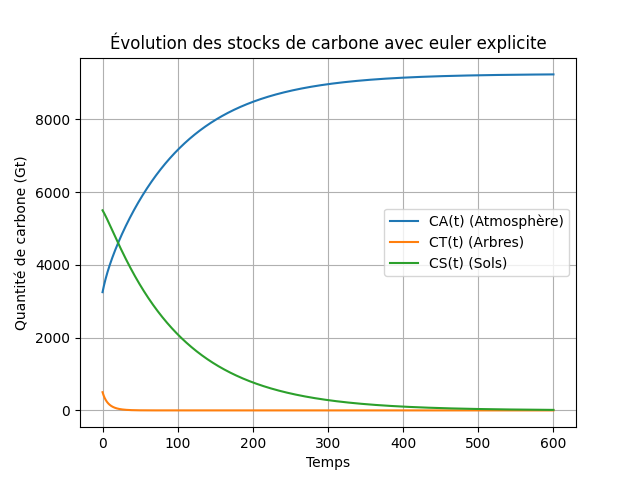
\includegraphics[width=\linewidth]{images/Euler_Explicite.png}
			
		\end{minipage}
		\caption{Solutions de nos méthodes}
		
	\end{figure}
	\newpage
	
	Comme on peut le voir tout nos implémentations se rapproche fortement du résultat du solveur.
	
	\textbf{Mais comment savoir laquelle de nos méthodes est la meilleure ? }
	
	Pour cela on commence par comparer la complexité respective de nos programmes.
	\begin{itemize}[label*=\textbullet]
		\item \textsc{Euler explicite} : $O(n)$
		\item \textsc{Euler implicite} : $O(m\times n)$
		\item \textsc{Adams-Bashforth} : $O(n)$
		\item \textsc{Runge-Kutta 2 (Heun)} : $O(n)$
	\end{itemize} 
	
	Dans un deuxième temps on peut s'intéresser à la stabilité de la méthode avec des pas temporel $h$ différents, auxquelles cas on a :
	

	
	\begin{figure}[h!]
		\centering
		
		% Première ligne
		\begin{minipage}[b]{0.45\textwidth}
			\centering
			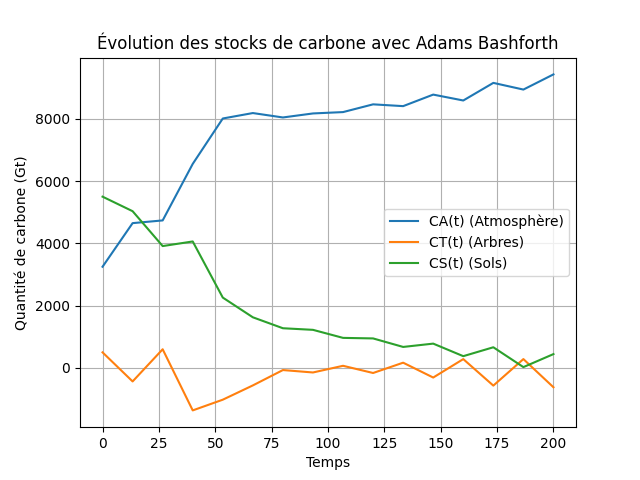
\includegraphics[width=\linewidth]{images/stabilite_adams_bashforth.png}
		\end{minipage}
		\hfill
		\begin{minipage}[b]{0.45\textwidth}
			\centering
			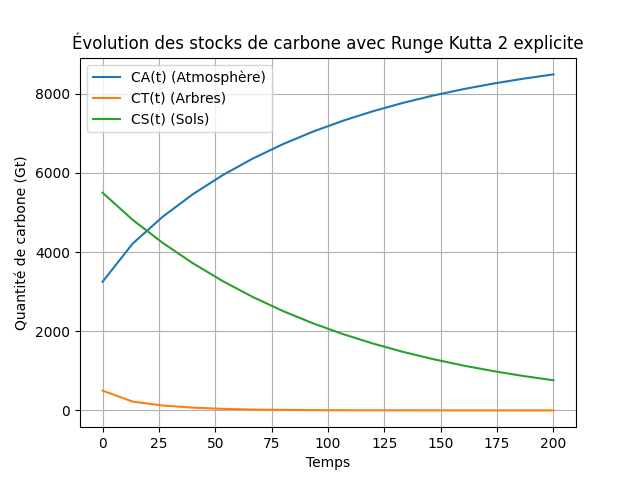
\includegraphics[width=\linewidth]{images/stabilite_runge_kutta.png}
		\end{minipage}
		
		\vspace{0.5cm}
		
		% Deuxième ligne
		\begin{minipage}[b]{0.45\textwidth}
			\centering
			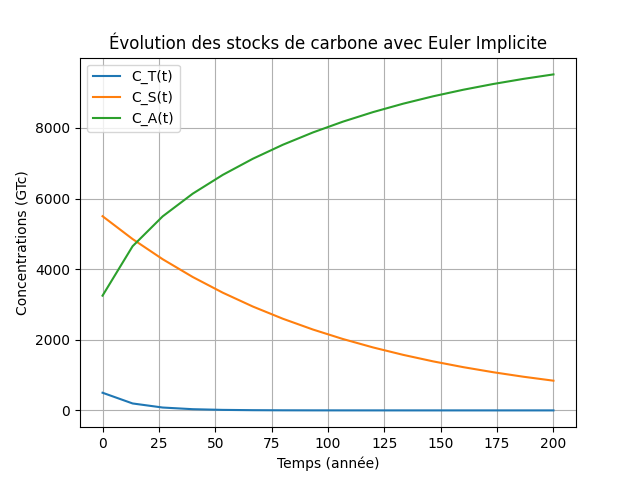
\includegraphics[width=\linewidth]{images/stabilite_euler_implicite.png}
		\end{minipage}
		\hfill
		\begin{minipage}[b]{0.45\textwidth}
			\centering
			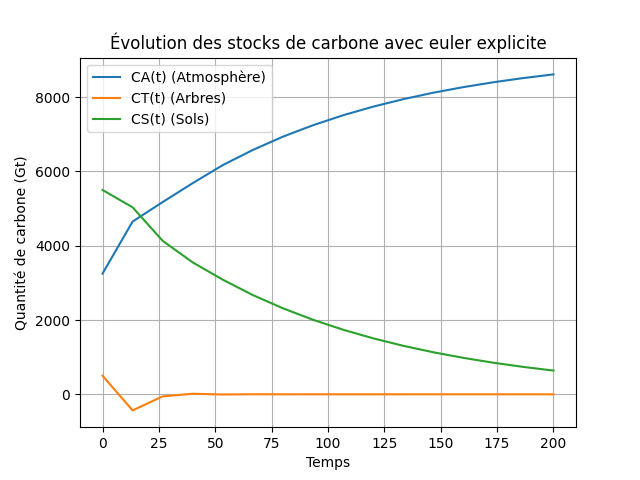
\includegraphics[width=\linewidth]{images/stabilte_euler_explicite.png}
		\end{minipage}
		\caption{Stabilité des méthodes par $h$}
	\end{figure}

	
		La méthode d'Adams-Basforth et d'Euler explicite sont plutôt sensible aux variations de $h$ ce qui en fait des méthodes peu stables.
	
		
		De plus au niveau des temps d'exécution des programmes on a : 
		\begin{itemize}[label*=\textbullet]
			\item \textsf{Euler explicite} : $0.029467344284057617$ s
			\item \textsf{Euler implicite} : $0.03226876258850098$ s 
			\item \textsf{Adams-Bashforth} : $0.14442753791809082$ s
			\item \textsf{Runge-Kutta 2} : $0.14023447036743164$ s
		\end{itemize}
		
		Par élimination avec la complexité computationelle, on considère que la méthode de Heun offre le meilleur compromis entre stabilité et vitesse de convergence. 
		Ainsi on prendra cette méthode dans la suite pour réaliser l'analyse paramétrique.
		
	
	
	
	\section{Analyse paramétrique}
	Observons maintenant l’impact de chaque paramètre ($\alpha$, $\beta$, $\gamma$, $\delta$, $K$) sur la séquestration du carbone.
	%On désire maintenant analyser l’impact des différents paramètres ($\alpha$, $\beta$, $\gamma$, $\delta$, $K$)  sur la séquestration du carbone. 
	%Pour cela on décide d'implémenter à notre algorithme \textbf{ALGO} qui prendra différentes valeurs pour chaque paramètres et tracera les différentes courbes afin de les comparer et finalement choisir le meilleur paramétrage.
	
	
	\begin{figure}[htbp]
	\centering
	\begin{minipage}[h]{0.9\linewidth}
		\centering		
		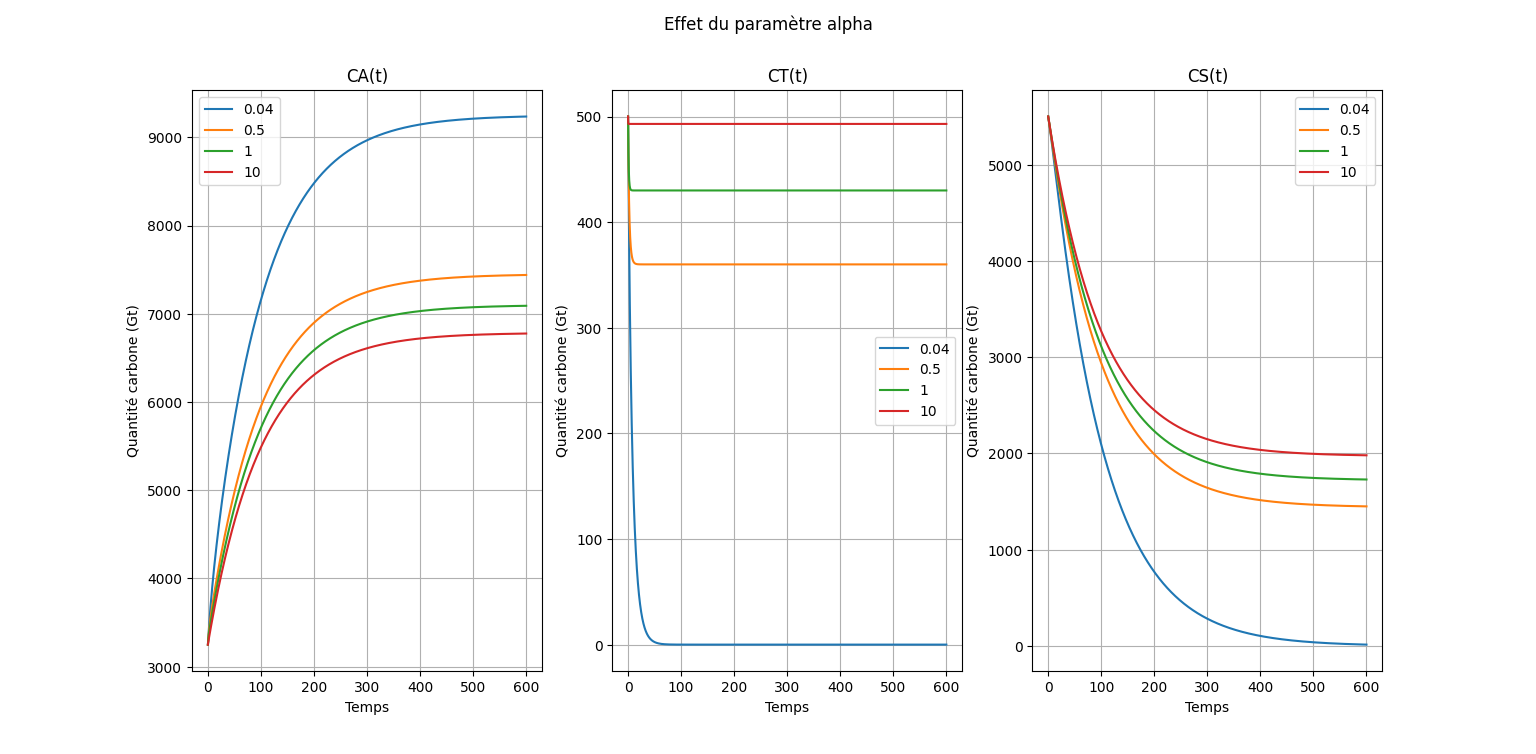
\includegraphics[width=\linewidth]{images/alpha_var.png}
		\par\vspace{0.5em}
		
		
		On a fait en sorte qu'$\alpha$ prenne ses valeurs dans $\acc{0.04,\hspace{2mm} 0.5,\hspace{2mm} 1,\hspace{2mm} 10}$.
		\begin{itemize}[label*=\textbullet]
			\item $C_{A}$ diminue lorsque $\alpha$ augmente, ce qui est logique étant donné que si le taux de séquestration de CO\textsubscript{2} dans les arbres augmentent alors la quantité de CO\textsubscript{2} dans l'atmosphère diminue.
			\item $C_{T}$ augmente proportionnellement à $\alpha$ ce qui est naturel étant donné que $C_{T}$ retrace la quantité de carbone stockée dans les arbres.
			\item $C_{S}$ augmente également proportionnellement à $\alpha$, on peut supposer que c'est un effet dû aux racines des arbres dans le sol.
		\end{itemize}
	\end{minipage}
	\end{figure}
	
	\begin{figure}[htbp]
	\centering
	\begin{minipage}[h]{0.9\linewidth}
		\centering
		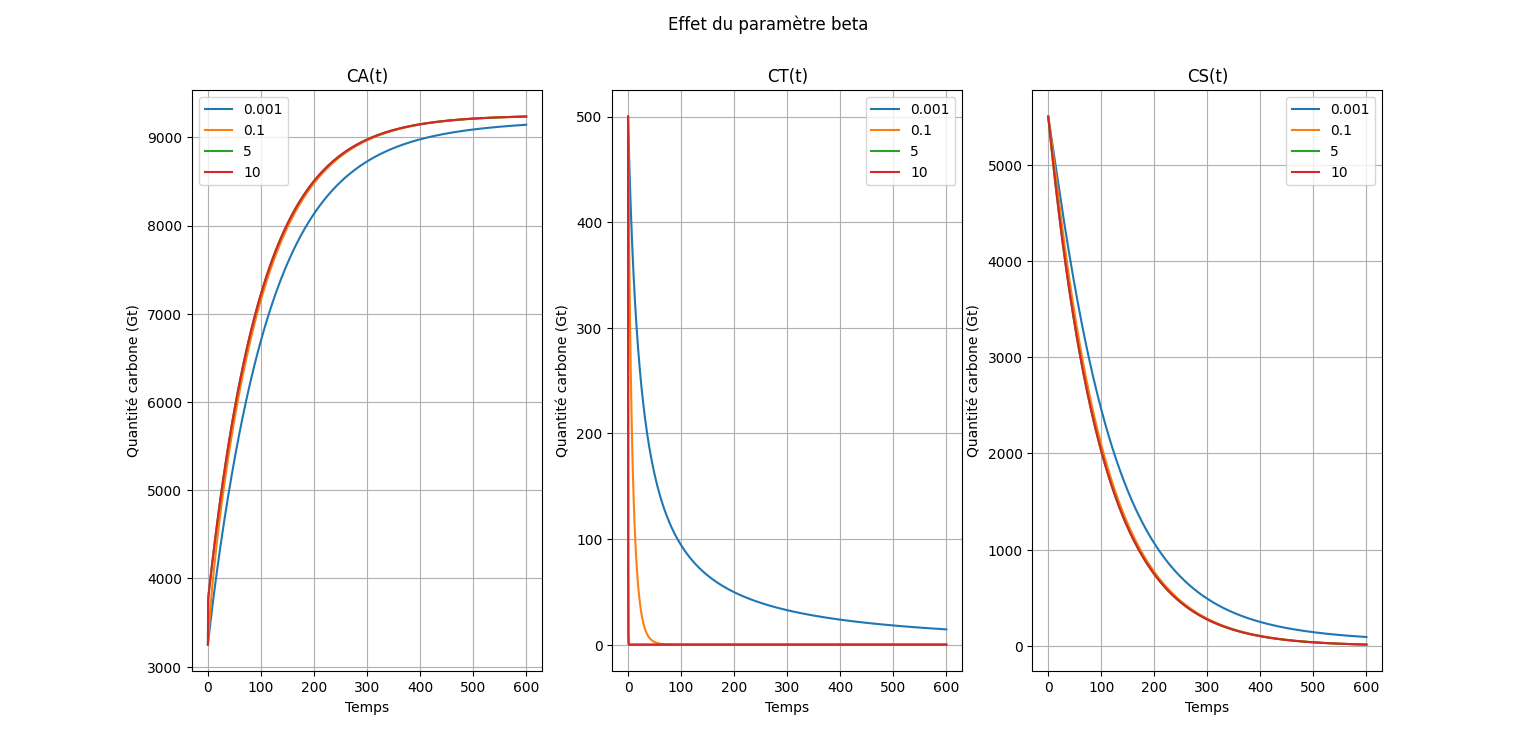
\includegraphics[width=\linewidth]{images/beta_var.png}
		\par\vspace{0.5em}
		
		
		Soit $\beta \in \acc{0.001,\hspace{1mm} 0.1,\hspace{1mm} 5,\hspace{1mm} 10}$.
		On observe que :
		\begin{itemize}[label*=\textbullet]
			\item $C_{A}$ augmente lorsque $\beta$ augmente ce qui est normal étant donné que $\beta$ relate de la respiration des arbres dans l'atmosphère. 
			\item $C_{T}$ décroit lorsque $\beta$ croît, cela vient du fait que $\beta$ représente le taux de libération du carbone des arbres vers l'atmosphère.
			\item On peut en tirer la même conclusion pour $C_{S}$, puisque les racines des arbres stockant du CO\textsubscript{2} en libère plus $\beta$ est grand.
		\end{itemize}
	\end{minipage}
	
	\end{figure}
	
	\begin{figure}[h]
		\centering
			\begin{minipage}[h]{\linewidth}
			\centering
			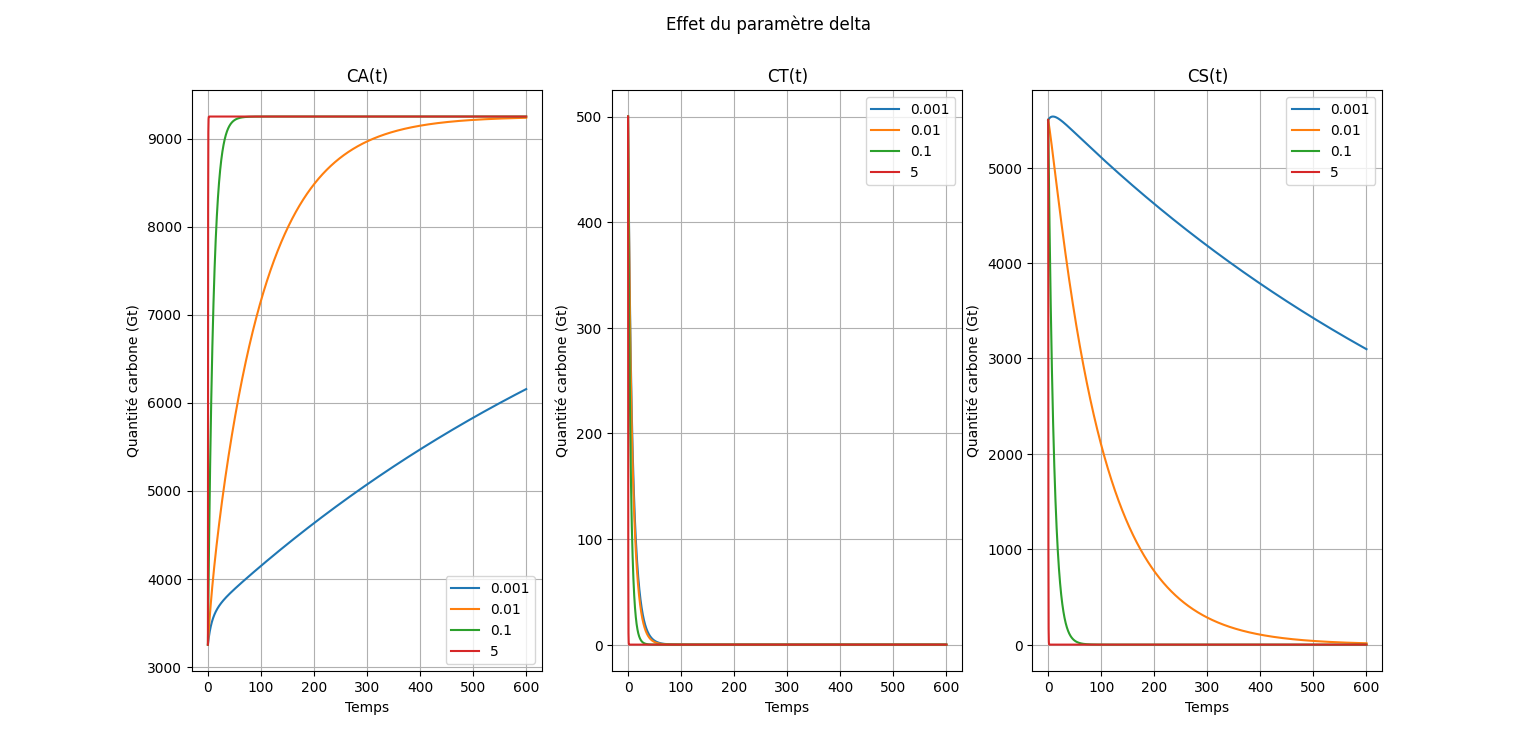
\includegraphics[width=\linewidth]{images/delta_var.png}
			\end{minipage}
			\par\vspace{0.5em}
			
			Soit $\delta \in \acc{0.0001,\hspace{1mm} 0.01,\hspace{1mm} 0.1,\hspace{1mm} 5} $.
			
			Etant donné que $\delta$ représente le taux de décomposition du carbone des sols et des arbres vers l'atmosphère. On comprends que plus $\delta$ augment, alors $C_{A}$ aussi. En revanche ce sera le contraire pour $C_{T}$ et $C_{S}$.
			
	\end{figure}
	
	\begin{figure}[h]		
		\centering
			\begin{minipage}[h]{\linewidth}
				\centering
			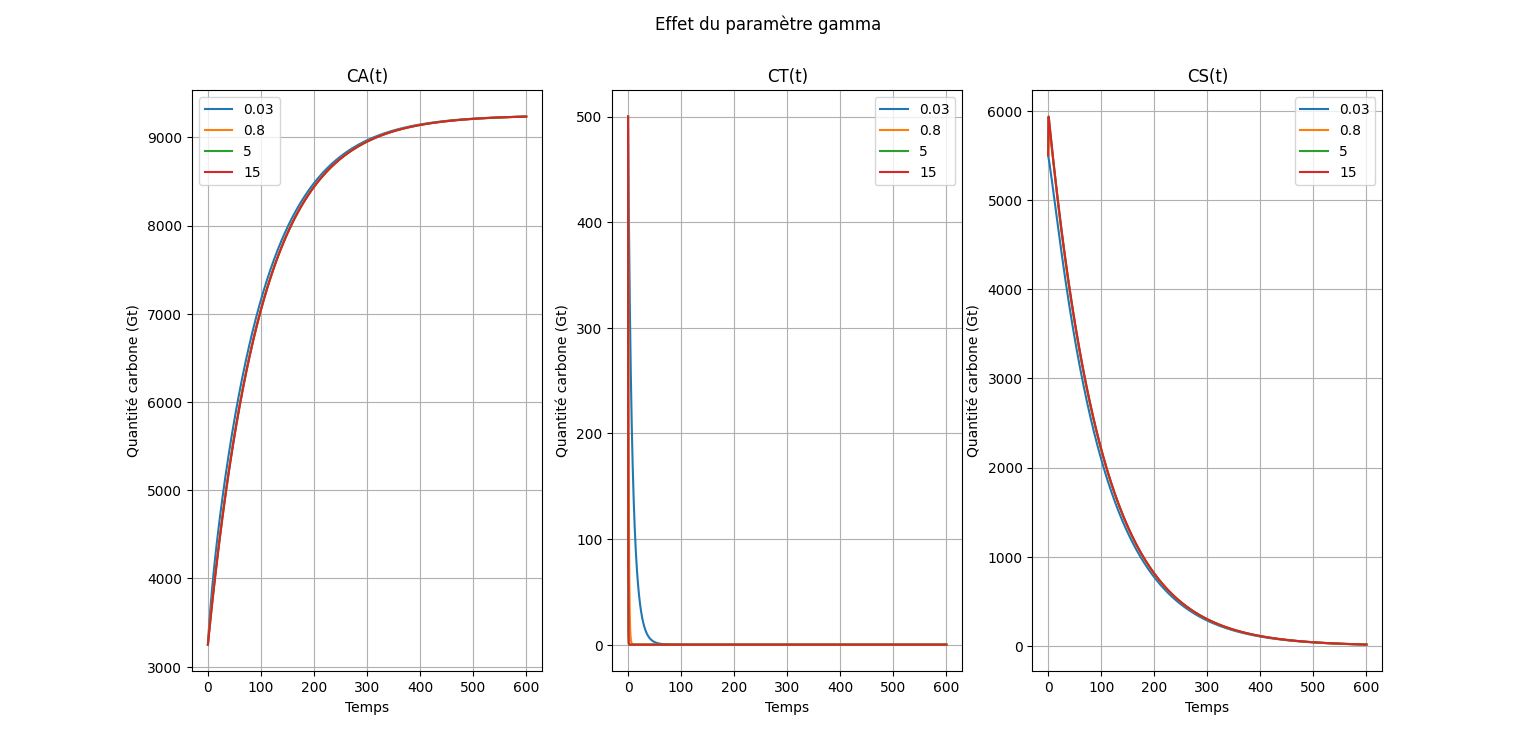
\includegraphics[width=\linewidth]{images/gamma_var.png}
			\end{minipage}
			\par\vspace{0.5em}
			
			
			Soit $\gamma \in \acc{0.03,\hspace{1mm} 0.8,\hspace{1mm} 5,\hspace{1mm} 15} $.
			
			On observe que :
			\begin{itemize}[label*=\textbullet]
				\item Une légère diminution de $C_{A}$ lorsque $\gamma$ augmente . 
				\item $C_{T}$ diminue fortement lorsque $\gamma$ croît puisque ce paramètre représente le taux de transfert de carbone des arbres vers le sol. 
				\item Donc $C_{S}$ croît lorsque $\gamma$ croît.
			\end{itemize}
	\end{figure}
		

	

	
	
	\clearpage
	
	\section{Répartition du travail}
		Au départ on s'est mit d'accord sur le type de résolution qu'on aller chercher.
		
		Puis nous nous sommes donnés à chacun des paquets d'implémentation de 3 méthodes à coder. Puis nous avons tous rassemblés et nous avons préparé le rapport et la soutenance ensemble. On s'est beaucoup entraidé pour la résolution de nos programmes respectif.
	
	\section{Conclusion}
	
	
	Le modèle serait plus réaliste si on prenait en compte l'effet des océans sur la séquestration du carbone également. Puisqu'il faut savoir que le phytoplancton transforme le CO2 atmosphérique en particules organiques dont une partie chute ensuite en profondeur. Il faudrait donc ensuite transformer le système en ajoutant $C_{O}(t)$ qui modéliserait la quantité de carbone stocké dans les océans. Le modèle serait plus précis puisque les océans intéragissent également avec les sols l'atmosphère et à certa ins endroits sur Terre même avec les arbres, il suffit de prendre l'exemple des mangroves sur certains littoraux ou encore des arbres bordant des fleuves.
	
	\bibliographystyle{IEEEtran}
	\bibliography{references}


\end{document}